\problemname{}

\illustration{0.29}{bill}{
    Bill Poucher (ICPC Executive Director, on the right).\\\textcopyright{} \href{https://www.huawei.com/en/news/2024/10/icpc-challenge-championship}{Huawei}, used with permission
}

Last week, Bill filled a champagne fountain for the first time.
Delighted by the champagne pouring from one glass into another, he decided that he wants to organize an even bigger champagne fountain for the next World Finals.
He already ordered $n$ glass bowls with different capacities to stack on top of each other to form a huge glass fountain.
However, he is still unsure how to pour the champagne into the fountain.
One bottle will not be enough and just pouring from the top might not fill every bowl.
Bill wants to try out different ways to fill the fountain, but wasting any champagne would be such a shame.

\begin{figure}[!h]
	\centering
	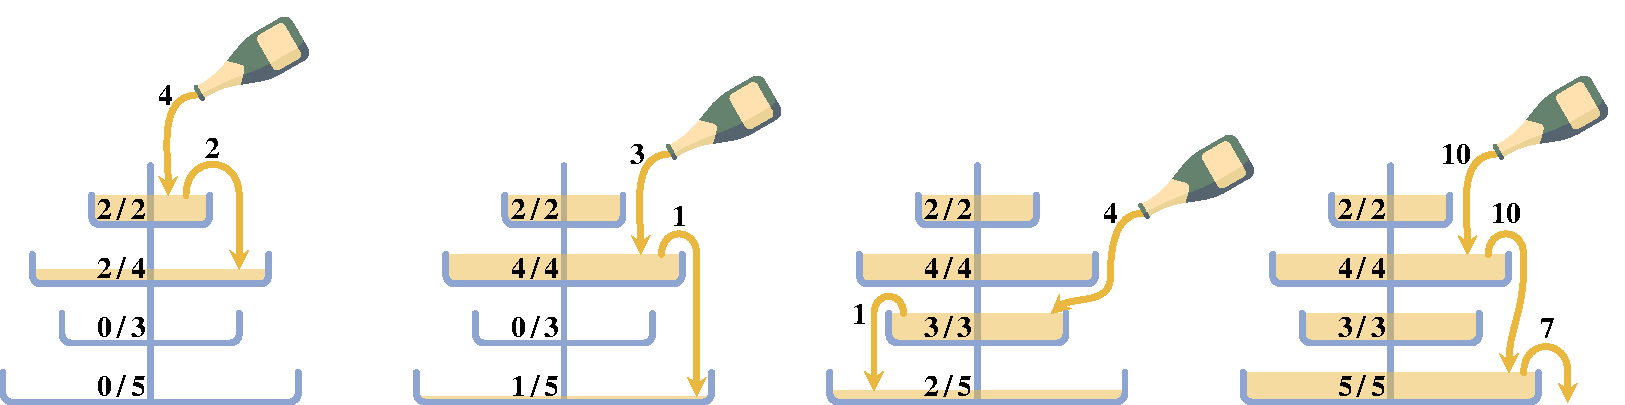
\includegraphics[width=0.95\textwidth]{sample.pdf}
	\caption{Illustration of Sample Input 2.
		The $i$th image visualizes the $i$th query of type~`\texttt{+}'.}
\end{figure}

This is your time to shine!
You are tasked with writing a program that simulates the process of pouring champagne into a given fountain.
With this program, Bill can now pretend to pour certain amounts of champagne into different levels.
If a bowl in some level is already filled up, then the champagne spills over to
the first level below it with larger capacity.
If the next larger level is also filled, the champagne spills over even further until eventually seeping into the ground, wasting the good champagne.
Additionally, Bill also wants to know at some times during the simulation process how much champagne currently is in a certain level.
%More formally, you are given the capacities of the bowls and have to process two types of queries:
%\begin{itemize}
%	\item[+] pour $x$ litres of champagne into level $\ell$.
%	\item[?] print the amount of champagne in level $\ell$.
%\end{itemize}

\section*{Input}
The input consists of:
\begin{itemize}
    \item One line with two integers $n$ and $q$ ($1\leq n, q \leq 3 \cdot 10^5$), the number of levels and the number of queries.
    \item One line with $n$ distinct integers $c$ ($1\leq c \leq 10^9$), the capacity of each level in litres.
    The levels are given in order from top to bottom.
    \item $q$ lines, each describing a query.
    The first symbol $t$ ($t \in \{\text{`\texttt{+}'}, \text{`\texttt{?}'}\}$) describes the type of the query.
    The format of the rest of the line depends on $t$:
    \begin{itemize}[leftmargin=1.95cm]
	    \item[$t=\text{`\texttt{+}'}$:] Two integers $\ell$ and $x$ follow ($1 \leq \ell \leq n$, $1 \leq x \leq 10^9$), the level into which Bill wants to pour $x$ litres of champagne.
	    \item[$t=\text{`\texttt{?}'}$:] One integer $\ell$ follows ($1 \leq \ell \leq n$), the level for which Bill requests the current amount of champagne in litres.
    \end{itemize}
    It is guaranteed that there is at least one query of type `\texttt{?}'.
\end{itemize}

\section*{Output}
For each query of type `\texttt{?}', output the amount of champagne in the requested level in litres.
